\chapter{Higgs mechanism and Supersymmetry}

\section{Introduction}
The Standard Model (SM) of particle physics has proved to be one of the most successful theories in physics. There are many good overviews of the SM, including~\cite{HALZEN} and~\cite{GRIFFITHS}. This chapter focuses on one of the less satisfactory elements of the Standard Model the origin of particle mass, for reasons that will be discussed later. It describes a proposed solution, concentrating on elements that are pertinent to the experimental study presented at the end of this thesis.

The Standard Model describes spin-1/2 matter particles, known as fermions, and their interactions mediated via the exchange of spin-1 particles, known as bosons (with the exception of gravity, which is mediated via a spin-2 boson). The bosons include the photon ($\gamma$), which mediates the electromagnetic force, the $\mathrm{W^{\pm}}$ and Z, responsible for the weak force, gluons, responsible for the strong force, and gravitons that mediate gravity.

In the Standard Model particle wavefunctions are invariant under local phase (gauge) transformations, a principle known as local gauge symmetry. The requirement for fermions to be invariant under the U(1) local gauge transformation results in the coupling of fermions and massless photons, i.e. electromagnetism. Similarly SU(2) and SU(3) invariance forms the basis of the weak and strong forces.

The Standard Model unifies the electromagnetic and weak forces with the electroweak theory of Glashow, Weinberg and Salam~\cite{Salam:1964ry}. This theory states that both forces are representations of the same fundamental process. Two new charges are introduced, weak isospin (T) and hypercharge (Y), which together with four new fields, $\mathrm{W^{1,2,3}_{\mu}}$ and B are invariant under SU$(2)_\mathrm{L}$ $\times$ U$(1)_{\mathrm{Y}}$, where L signifies that only left-handed particles take part in the weak interaction. These fields mix to form the $\gamma$ (represented by the field A), $\mathrm{W^{\pm}}$ and Z:

\begin{equation}
	A_{\mu} = B_{\mu} \cos{\theta_{W}} + W_{\mu}^{3} \sin{\theta_{W}}
	\label{eqn:A}
\end{equation}
\begin{equation}
	W_{\mu}^{\pm} = \frac{1}{\sqrt{2}}(W_{\mu}^{1} \mp W_{\mu}^{2})
	\label{eqn:W}
\end{equation}
\begin{equation}
	Z_{\mu} = - B_{\mu} \sin{\theta_{W}} + W_{\mu}^{3} \cos{\theta_{W}}
	\label{eqn:Z}
\end{equation}

%\begin{equation}
%	W_{\mu}^{3} = A^{\mu}\sin{\theta_{W}} + Z^{\mu}\cos{\theta_{W}}
%	\label{eqn:Z}
%\end{equation}

where $\theta_{W}$ is the Weinberg angle. 

The local gauge invariance that introduced the massless photon has a similar effect on all the bosons and thus requires them all to be massless. However experiment has shown that both the $\mathrm{W^{\pm}}$ and Z are massive. The introduction of explicit mass terms for these fields destroys gauge invariance, which is the foundation of the SM. The Higgs mechanism~\cite{citeulike:918519} represents a possible solution to this problem.

%A source for particle masses is presented along with a further problem that this introduces. A solution to this problem is given by a theory known as Supersymmetry (SUSY). This chapter describes SUSY and elements of the theory that impact on the experimental search presented later.   

%one problem with...

\section{Higgs mechanism}
%The standard model (SM) of particle physics has proved extremely successful at describing the electro-weak and strong interactions. One of its major limitations is the need to explain the massive vector bosons, $\mathrm{W^{\pm}}$ and Z. Introducing explicit mass terms destroys the Lagrangians gauge invariance, making the theory un-renormalisable. The Higgs mechanism is a means for giving the $\mathrm{W^{\pm}}$ and Z mass while retaining gauge invariance. 

Boson masses may be introduced through a process known as spontaneous symmetry breaking, which occurs when the Lagrangian is invariant under local gauge transformations but the ground (vacuum) state is not. The electroweak $\mathrm{SU(2) \times U(1)_{Y}}$ symmetry must be broken to give mass to the $\mathrm{W^{\pm}}$ and Z whilst leaving the $\gamma$ massless. This can be accomplished with the addition of a complex scalar doublet, $\phi$:

\begin{equation}
	\phi = \binom{\phi^{+}}{\phi^{0}}
\end{equation}

%pic from Filip

%\begin{equation}
%	\phi = \phi_{1} + i \phi_{2}
%\end{equation}

%\begin{equation}
%	\phi^{*}\phi = \phi_{1}^{2} + \phi_{2}^{2}
%\end{equation}

The standard model Lagrangian gains additional terms:

\begin{equation}
	\mathcal{L} = D_{\mu}\phi^{*}D_{\mu}\phi - V(\phi) = D_{\mu}\phi^{*}D_{\mu}\phi + \mu^{2}\phi^2 - \lambda \phi^{4}
	\label{eqn:lagrangian}
\end{equation}
%1.21 filip

with the covariant derivative

\begin{equation}
	D_{\mu} \phi = (\partial_{\mu} + igW_{\mu}^{a}T^{a} + ig^{\prime}B_{\mu})\phi
\end{equation}

where $T^{a}$ is the $\mathrm{SU(2)}$ group generator and g(g$^{\prime}$) is the $W_{\mu}^a$ ($B_{\mu}$) coupling constant. $\mu$ and $\lambda$ are the $\phi$ mass parameter and self-interaction, respectively. The first term of Equation~\ref{eqn:lagrangian} describes the kinetic part of the Lagrangian and the last two terms the potential, V($\phi$).

%\begin{equation}
%	van der aa 1.3
%\end{equation}


%. Requiring the vacuum to be invariant under implies that $\phi$ is constant in the vacuum state. 

Two possible potential forms exist depending on the value of $\mu^2$, as shown in Figure~\ref{fig:Higgs_potential}. In the case of $\mu^{2} > 0$ the potential has a minima at $\phi = 0$. If $\mu^{2} < 0$ the minima form a circle where

\begin{figure}[bt]
  \centering
  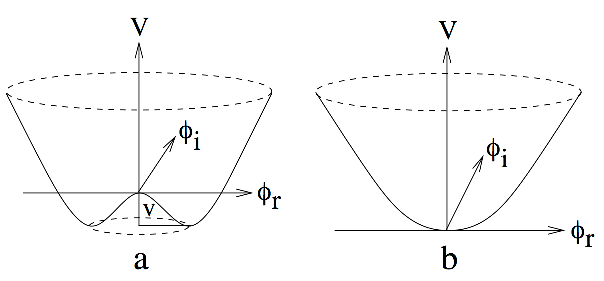
\includegraphics[width=0.55\textwidth]{theory/Higgs_potential}
  \caption{The Higgs potential as a function of a complex scalar field with negative (a) and positive (b) mass parameter. $\phi_{r}$ ($\phi_{i}$) represents the real (imaginary) component of $\phi$.
  \label{fig:Higgs_potential}}
\end{figure}

\begin{equation}
	\phi^2 = \frac{\mu^{2}}{2 \lambda} = \frac{v^2}{2} \qquad \mathrm{where\,} v = \frac{\mu}{\sqrt{\lambda}}
	\label{eqn:minima}
\end{equation}

%Once we have discovered the possible values for the minima we can expand about an arbitrary point on the circle. As the Lagrangian is invariant under rotations in the complex plane any value of $\theta$ may be taken, for convenience we choose $\theta$ = 0:
%.see van der AA 1.3

%The vacuum expectation value of $\phi$ is thus degenerate. The Goldstone theorem states that for 

We can then choose a vacuum expectation value (vev) for this field. The vev should be zero for the charged component of the $\phi$ field to preserve the electromagnetic, $\mathrm{U(1)_{EM}}$, symmetry. Expanding $\phi$ arbitrarily about its vev results in one massive and three massless bosons. The massless bosons are a result of the Goldstone theorem, which states that for each broken symmetry, a massless field will result. These particles are known as Goldstone bosons and the massive boson is known as the Higgs boson.

As the expansion is arbitrary we can choose the gauge such that the Goldstone bosons are eliminated. We can expand $\phi$ as:

%\begin{equation}
%	\phi = \frac{1}{\sqrt{2}}(\frac{\mu}{\sqrt{1}} + H + i\eta)
%	\label{eqn:expansion}
%\end{equation}

%The fields H and $\eta$ are fields with zero vacuum expectation value. Inserting~\ref{eqn:expansion} into~\ref{eqn:lagrangian} we can see that the field H gains a mass term

%\begin{equation}
%	m_{H} = v \sqrt{2 \lambda}
%\end{equation}

%While $\eta$ is a massless particle called a Goldstone boson. This massless particle is a direct consequence of the degenerate nature of the vacuum. 

%Egede thesis
%The Higgs mechanism has been developed to remove the Goldstone boson. To begin with the derivatives are replaced by their covariant forms. 

%One ground state is:

%\begin{equation}
%	\langle \phi \rangle = \frac{1}{\sqrt{2}} \binom{0}{v}
%\end{equation}

%where:

%\begin{equation}
%	v = \frac{\mu}{\sqrt{\lambda}}
%\end{equation}
	
%Instead of making an arbitrary choice of the minima we may choose it such that Goldstone boson is eliminated. 

\begin{equation}
	\phi(x) = e^{iT^{a}\theta_{a}(x)} \frac{1}{\sqrt{2}}\binom{0}{v + H(x)}
	\label{eqn:unitarygauge}
\end{equation}

Taking Equations~\ref{eqn:unitarygauge} and~\ref{eqn:lagrangian} together with the physical electroweak fields~\ref{eqn:A},~\ref{eqn:W} and~\ref{eqn:Z}, we obtain the masses:

%\begin{equation}
%	M_{W} = \frac{v g_{2}}{2} \\qquad M_{Z} = \frac{v}{2}\sqrt{g_{2}^{2} + g_{1}^{2}} \\qquad M_{A} = 0
%\end{equation}

\begin{equation}
	m_{W} = m_{Z} \cos{\theta_{W}} = \frac{gv}{2}, \qquad m_{A} = 0
\end{equation}

%As a consequence of this the gauge bosons acquire a mass. 

Thus the Higgs mechanism, by utilising spontaneous symmetry breaking and a convenient choice of gauge, gives mass to the $\mathrm{W^{\pm}}$ and Z while keeping the $\gamma$ massless.   

The Standard Model also requires a mechanism for explaining the fermion masses. These can be introduced by forming interaction terms between left-handed fermions, right-handed fermions and the Higgs field. These interactions are known as Yukawa couplings. However, for each interaction a new coupling constant is required, the values of which are not predicted.

More of a problem with the Higgs mechanism is that of the Higgs mass itself. The physical mass ($m_{H}$) is related to the the bare mass ($m_{H_{0}}$) with corrections from loop diagrams ($\Delta m_{H}$), as illustrated in Figure~\ref{fig:Higgs_correction}.

\begin{equation}
	m_{H}^2 = m_{H_{0}}^{2} + \Delta m_{H}^2
\end{equation}

The fermion contribution to the correction is:

\begin{equation}
	\Delta m_{H}^{2} \approx O(-\Lambda^{2})
\end{equation}

where $\Lambda$ represents the scale where new physics is introduced and the theory no longer holds. If no new physics occurs at high energy scales then the cut-off becomes the Planck scale, $10^{19}$\GeVcc. An upper limit on the Higgs mass can be determined from the WW scattering crosssection which at high energies becomes greater than unitarity for $m_{H} > 1\TeVcc$~\cite{citeulike:918524}. To cancel the correction and result in the Higgs boson mass of $\sim1\TeV$ the bare mass must be $\approx 10^{19} \GeVcc$. While mathematically possible this is aesthetically displeasing and is known as the fine tuning problem.

\begin{figure}[bt]
  \centering
  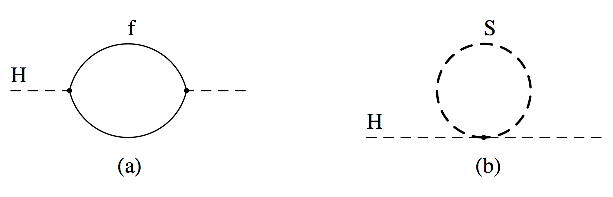
\includegraphics[width=0.5\textwidth]{theory/Higgs_correction}
  \caption{Corrections to the Higgs mass from fermion (a) and boson (b) loops.~\cite{citeulike:681336}
  \label{fig:Higgs_correction}}
\end{figure}

As well as corrections from fermions, boson loops also contribute. Their contribution takes the same form as the fermion loops but with the opposite sign. Thus if a theory could be formed that matches fermions and bosons the correction would be:

\begin{equation}
	\Delta m_{H}^{2} \approx O(m_{B}^2 - m_{f}^2)
\end{equation}

which is less than $m_{H}^2$ if the fermion and boson partners have similar masses:

\begin{equation}
	m_{B}^2 - m_{F}^2 < 1 \TeVcc
\end{equation}

This indicates new physics below 1\TeV that may take the form of the theory described above. One such theory is supersymmetry.

\section{Supersymmetry}
Supersymmetry (SUSY) is a theory that relates fermions to bosons. An operator (Q) is proposed that transforms the two types:

\begin{equation}
	Q|boson\rangle = |fermion\rangle \qquad Q|fermion\rangle = |boson'\rangle
\end{equation}

As derived in~\cite{citeulike:681336} the Q operator obeys the following anti-commutation rule

\begin{equation}
	\{ Q_{\alpha}, Q_{\beta}^{\dagger} \} = 2\sigma^{\mu}_{\alpha \beta}P^{\mu}
\end{equation}

where $P^{\mu}$ is the generator of the space-time translation and $\sigma$ the Pauli matrices. Supersymmetric states are grouped together into supermultiplets, which contain a fermion and boson. These are related by the Q operator, with the particles known as each other's superpartner. It can be shown that the mass operator $P^{2}$ commutes with Q and thus that the superpartners have equal mass~\cite{citeulike:681336}. Also the Q operator commutes with the gauge symmetries therefore the superpartners must have equal charge, weak isospin, hypercharge and colour. 

It is clear that no superpartners of any known particles have been discovered with the same mass and quantum numbers except spin, hence supersymmetry must be broken. This is possible because the superpartners of the Standard Model particles may have an explicit mass term in their Lagrangian without violating electroweak symmetry~\cite{citeulike:681336}. The Supersymmetry breaking mechanism is not understood and most phenomenological models parameterize it.

\section{The Minimal Supersymetric Standard Model \label{sec:mssm}}
The Minimal Supersymmetric Standard Model (MSSM) is the simplest supersymmetric extension to the standard model that aims to minimise the numbers of superfields and interactions. For each SM particle a new superpartner is required.

Two Higgs doublets with different hypercharge are required to give mass to the up and down type fermions: 

\begin{equation}
	\phi_{u} = (\phi_{u}^{+}, \phi_{u}^{0}) \qquad \phi_{d} = (\phi_{d}^{0}, \phi_{d}^{-}) 
\end{equation}

The vev of these fields may be written:

\begin{equation}
	\langle \phi_{u}\rangle = \binom{0}{v_u} \qquad \langle \phi_{d}\rangle = \binom{v_d}{0}
\end{equation}

These can be related to the $\mathrm{W^{\pm}}$ mass via:

\begin{equation}
	v_{u}^{2} + v_{d}^{2} = \frac{2m_{W}^{2}}{g} \approx (174 \GeVcc)^{2}
\end{equation}

The ratio of the two vev's is not predicted, and we define this ratio as:

\begin{equation}
	\tan\beta = \frac{v_u}{v_d}
\end{equation}

After $\mathrm{SU(2) \times U(1)_{Y}}$ symmetry breaking three of the Higgs degrees of freedom are taken by the $\mathrm{W^{\pm}}$ and Z, leaving five massive Higgs bosons: a charge parity (CP) symmetry odd neutral scalar $A$, two CP even neutral scalars $h$ and $H$ and a pair of charged scalars $H^{+}, H^{-}$:

\begin{equation}
	A = \sqrt{2}(\cos{\beta}\ \mathrm{Im}[\phi^{0}_{u}] + \sin{\beta}\ \mathrm{Im}[\phi^{0}_{d}])
\end{equation}
\begin{equation}
	H^{\pm} = (\cos{\beta}\ \phi^{\pm}_{u} + \sin{\beta}\ \phi^{\mp*}_{d})
\end{equation}
\begin{equation}
	\left(
	\begin{array}{c}
		h \\
		H \\
		\end{array} \right) = \sqrt{2} \left(
	\begin{array}{cc} 
		\cos{\alpha} & -\sin{\alpha} \\ 
		\sin{\alpha} & \cos{\alpha} \\ 
	\end{array} 
	\right)
	\left( \begin{array}{c} 
		\mathrm{Re} [H_{u}^{0}] - v_u\\ 
		\mathrm{Re} [H_{d}^{0}] - v_d \\
	\end{array}
	\right)
\end{equation}

The mixing angles $\alpha$ and $\beta$ are determined at tree level by:

\begin{equation}
	\cos^2{(\beta - \alpha)} = \frac{m_h^2(m_Z^2 - m_h^2)}{m_A^2(m_H^2 - m_h^2)}
	\label{eqn:alpha}
\end{equation}

%\subsection{Theoretical constraints}
Theoretical constraints can be applied to $\beta$ as the fermions masses are determined by Yukawa couplings. The requirement that fermion masses do not diverge leads to the constraint $1.2 \lesssim \tan{\beta} \lesssim 60$.~\cite{kane:2002}

At tree level the Higgs masses depend only on two parameters, $m_{A}$ and $\tan{\beta}$:
\begin{equation}
	m_{H^{\pm}}^2 = m_{A}^2 + m_{W}^2
\end{equation}
\begin{equation}
	m_{h,H}^2 = \frac{1}{2}\left( m_{A}^2 + m_{Z}^2 \mp 
	\sqrt{(m_{A} + m_{Z})^2 - 4m_{Z}^2 m_{A}^2 \cos{2\beta})}
	\right)
	\label{eqn:m_h}
\end{equation}

From~\ref{eqn:m_h} one can obtain an upper bound on $m_{h}$:

\begin{equation}
	m_{h} \le m_{Z}|\cos{2\beta}|
\end{equation}

However loop corrections modify this. The maximum one loop contribution is

\begin{equation}
	m_{h}^2 \lesssim m_{Z}^2 + \frac{3g^2m_{t}^4}{8\pi^2m_{W}^2} 
	\left[ 
	  \ln \left( \frac{M_{S}^2}{m_{t}^2} \right) + \frac{X_{t}^2}{M_{S}^2} 
	    \left( 1 - \frac{X_{t}^2}{12 M_{S}^2} \right)
	\right] 
\end{equation}

where $M_{\mathrm{SUSY}} = M_{\tilde{t}} = M_{\tilde{b}}$, $M_{S}^2 = M_{\mathrm{SUSY}}^2 + m_{t}^2$ and $X_{t} = (A_{t} - \mu \cot{\beta})$.\footnote{A tilde indicates the superpartner of the indicated particle.} $\mu$ is the Higgs mixing parameter and $A_t$ the trilinear Higgs-$\tilde{s}$ coupling. This correction increases with $X_t$ reaching its maximal value, \mhmax, at $X_t = \sqrt{6}M_S$:

\begin{equation}
	\mhmax \lesssim 130 \GeVcc
\end{equation}

This number is calculated with a top mass of 175\GeVcc and assuming that no superpartner masses ($M_{\mathrm{SUSY}}$) exceed 1\TeVcc. 

Two Higgs mass regimes may be identified depending on the ratio of $m_{A}$ and \mhmax:

\begin{itemize}
	\item $m_{A} \gg \mhmax$: $m_A \sim m_H \sim m_{H^{\pm}}$ with h behaving like the SM Higgs.
	\item $m_{A} \ll \mhmax$: $m_A \sim m_h$ with H behaving like the SM Higgs.
\end{itemize}

The couplings of the MSSM Higgs sector compared to the SM are shown in Table~\ref{tab:MSSMcoupling}. It can be seen that the h and H bosonic couplings are greatly suppressed compared to the SM couplings. In the two mass regimes the couplings simplify. For large $m_{A}$ one can derive from Equation~\ref{eqn:alpha} that $\cos(\beta - \alpha) \ll 1$. This implies that $h$ coupling to bosons will be similar to the SM Higgs boson and the boson couplings of the $H$ will be strongly suppressed, while the coupling of both the $A$ and $H$ will be enhanced by a factor $\tan{\beta}$ for down-type fermions. This may prove useful in experimental searches where down-type final state particles are sought. This is especially true in the case of  b quarks and $\tau$ leptons since the Higgs coupling is proportional to mass.

\begin{table}[tbp]
	\centering
	\begin{tabular}{|l|c|c|c|}
	\hline
	coupling & $h$ & $H$ & $A$ \\ \hline
	up-type fermions & $\cos{\alpha} / \sin{\alpha}$ & $\sin{\alpha} / \sin{\beta}$ & $\cot{\beta}$ \\ \hline
	down-type fermion & $- \sin{\alpha} / \cos{\beta}$ & $\cos{\alpha} / \cos{\beta}$ & $\tan{\beta}$ \\ \hline
	W,Z & $\sin{(\beta - \alpha)}$ & $\cos{(\beta - \alpha)}$ & 0 \\ \hline
	\end{tabular}
\caption{MSSM couplings for the neutral Higgs bosons.\label{tab:MSSMcoupling}}
\end{table}

\section{Summary}
The Higgs mechanism provides a means for giving mass to the $\mathrm{W^{\pm}}$ and Z bosons. Various problems have been identified with the Higgs mechanism that supersymmetric theories aim to solve. The MSSM is the simplest supersymetric extension to the Standard Model and the phenomenology of its Higgs sector has been explained. Neither Higgs bosons nor any supersymmetric particles have so far been discovered. They are the prime targets of the next generation of particle experiments and if they exist with masses $< 1\TeVcc$ they should be seen at LHC.